As mentioned above, a dynamic programming allowing to solve the pricing problems for Ryan \& Foster method and diving heuristics have also been studied. However, due to their complexity, the have not been implemented successfully. In the following section, we present how it could have been possible to improve the BnP algorithm using these methods.

\subsection{Dynamic programming for Ryan \& Foster branching rule}
\label{dynamic_rf}

As mentioned in \ref{generic}, we can use dynamic programming to solve the subproblems for the generic branching method. Indeed, the branching rules simply fix variables so it is easy to preprocess the subproblem to put it under a classical knapsack problem. However, this is not possible for the Ryan \& Foster branching method. The constraints of type $x_i = x_j$ can be handled by creating a "super-object" corresponding to both $i$ and $j$, which ensure that the constraint is satisfied. But the constraints of type $x_i + x_j \leq 1$ cannot be handled easily. For this branching method, a knapsack problem with conflicts has to be solved. In \cite{sadykov2013bin}, a dynamic programming method is given.

The first thing to do is to extract a \textit{conflict graph} from the subproblem. The vertices correspond to the items in the problem and an edge is added between $i$ and $j$ as soon as there is a constraint $x_i + x_j \leq 1$. Each edge represents a conflict between two items. Once this graph is extracted, the method constructs the \textit{interval representation} of the conflict graph. It is possible to construct this representation in $o(|V| + |E|)$ \cite{corneil1998ultimate} for a conflict graph $G=(V,E)$ when such representation exists. In \cite{sadykov2013bin}, a method is also provided when the interval representation cannot be constructed.

\begin{figure}[!ht]
	\centering
	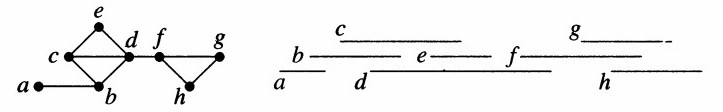
\includegraphics[width=0.8\linewidth]{img/conflict-graph.jpg}
	\caption{A conflict graph where each edge $(i,j)$ corresponds to a conflict between $i$ and $j$ and its interval representation. It is possible to assign at each interval a coordinate for its left and right endpoints.}
\end{figure}

Given the conflict graph $G=(V,E)$, where the vertex are indexed in non-decreasing order of the right endpoints of the corresponding intervals $\{I_i = (a_i , b_i)\}, \ i \in V$, associated to the subproblem. We can define 
\begin{equation*}
	Q_i = \{ j : \ j<i, \ (i,j) \notin E\} \qquad \text{and} \qquad prev_i = \begin{cases}
	\max \{j, \ j \in Q_i\} &\text{if }  Q_i \neq 0 \\
	0 &\text{if }  Q_i = 0
	\end{cases}
\end{equation*}
for all $i \in V$. The algorithm relies on two observations. The first is that for every pair $(i,j)$ such that $1 \leq j \leq prev_i$, $i$ and $j$ are not in conflict but if $prev_i < j < i$, then $i$ and $j$ are in conflict. If we note $P(i,c)$ the value of an optimal solution of the knapsack with conflict for the first $i$ items and a knapsack capacity $c$, the second observation is the following 
\begin{equation}
	\label{generic-dynamic}
	P(i,c) = \max \ \{P(prev_i,c-s_i) + p_i, \ P(i-1,c)\}
\end{equation}
where $s_i$ and $p_i$ are the size and the profit corresponding to the item $i$. Using \eqref{generic-dynamic}, we can compute iteratively the values $P(i,c)$ and the optimal value of the knapsack with conflict is given by $P(N,C)$. Then, it is possible to process a backtracking step as in \eqref{dynamic_rf} to recover the items involved in the optimal cost.